%%%%%%%%%%%%%%%%%%%%%%%%%%%%%%%%%%%%%%%%%
% Friggeri Resume/CV
% XeLaTeX Template
% Version 1.2 (3/5/15)
%
% This template has been downloaded from:
% http://www.LaTeXTemplates.com
%
% Original author:
% Adrien Friggeri (adrien@friggeri.net)
% https://github.com/afriggeri/CV
%
% License:
% CC BY-NC-SA 3.0 (http://creativecommons.org/licenses/by-nc-sa/3.0/)
%
% Important notes:
% This template needs to be compiled with XeLaTeX and the bibliography, if used,
% needs to be compiled with biber rather than bibtex.
%
%%%%%%%%%%%%%%%%%%%%%%%%%%%%%%%%%%%%%%%%%

\documentclass{friggeri-cv} % Add 'print' as an option into the square bracket to remove colors from this template for printing

\addbibresource{bibliography/publications.bib} % Specify the bibliography file to include publications

\begin{document}


\header{Malcolm}{Ramsay}{Computational Chemist} % Your name and current job title/field

%----------------------------------------------------------------------------------------
%	SIDEBAR SECTION
%----------------------------------------------------------------------------------------

\begin{aside} % In the aside, each new line forces a line break
    %\vspace{30 mm}~
\begin{flushleft}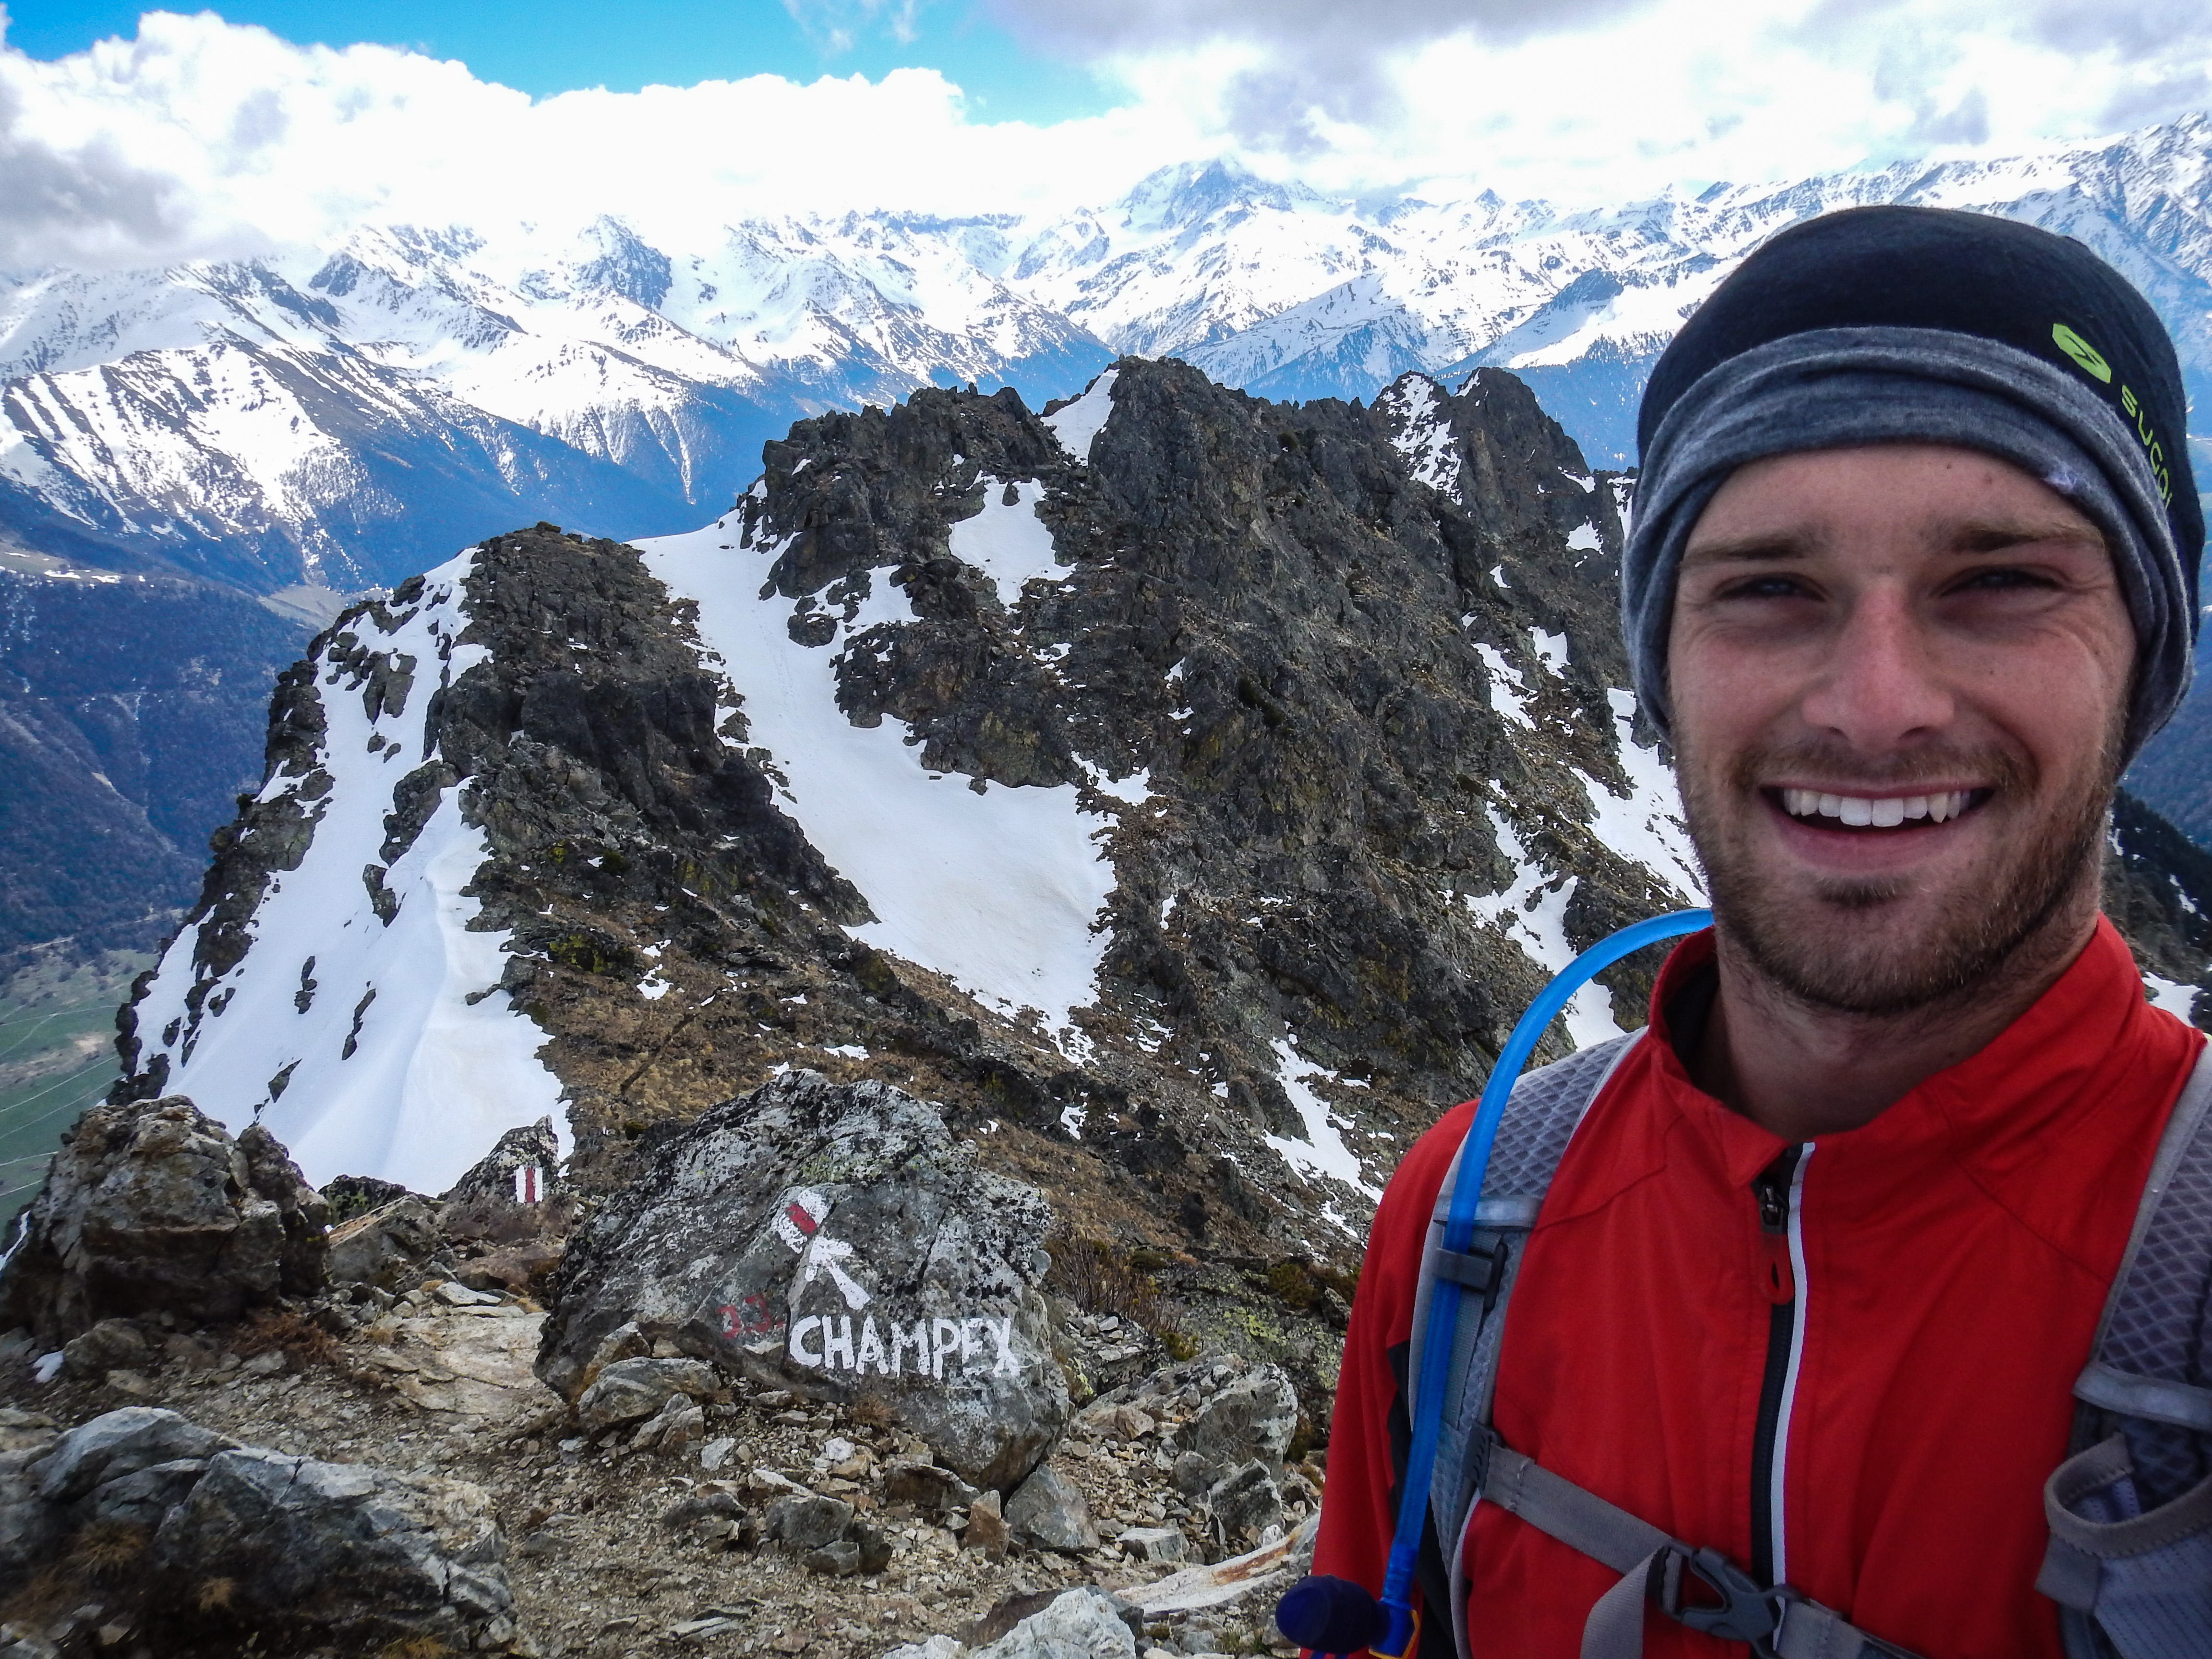
\includegraphics[width=\textwidth]{portrait}\\\end{flushleft}~
\section{Contact}
0466 224 898
\href{mailto:malramsay64@gmail.com}{malramsay64@gmail.com}
\href{github.com/malramsay64}{github.com/malramsay64}
\section{Programming}
Python, C++, C, \LaTeX,
Bash, Unix, Matlab, Git, 
GNU Make, Gnuplot, MPI,
Mathematica, Fortran
\end{aside}

%----------------------------------------------------------------------------------------
%	EDUCATION SECTION
%----------------------------------------------------------------------------------------

\section{Education}

\begin{entrylist}

%------------------------------------------------

\entry
{2009--2015}
{Bachelor of Science (Advanced) Honours}
{University of Sydney}
{I completed my honours project in Theoretical Chemistry under the supervision of Prof. Peter Harrowell and Dr. Asaph Widmer-Cooper gaining 1\textsuperscript{st} Class Honours and 1\textsuperscript{st} in my cohort. For my Honours project I utilised molecular dynamics simulations to model the growth of molecular crystals, using cluster computers to perform the long simulations. I attained majors in both Computational Science and Chemistry with a Distinction average over the course of my degree.
}

%------------------------------------------------

\entry
{2013--2014}
{Exchange Semester}
{The University of California, Santa Barbara}
{I undertook an academic exchange in the final semester of my degree, finishing the requirements for my Chemistry and Computational Science Majors.}

%------------------------------------------------

\entry
{2009}
{Chemistry Olympiad Summer School}
{}
{I spent two weeks at Monash University learning most 1\textsuperscript{st} year and some 2nd year Chemistry. I placed 11\textsuperscript{th} in the Australian Chemistry Olympiad, competing against the top high school chemistry students in Australia.}

\entry
{2004--2009}
{Higher School Certificate}
{Normanhurst Boys High School}
{In my final year at school I was awarded Senior Sportsman of the year, CALTEX All-rounder award, Buttfield Memorial Trophy for best and fairest in Open Soccer, Best and Fairest in 1st Grade Waterpolo. I was Age Champion in Swimming, Cross Country and Athletics for all of my six years at High School. My ATAR was 95.75.
}


\end{entrylist}


%----------------------------------------------------------------------------------------
%	PUBLICATIONS SECTION
%----------------------------------------------------------------------------------------

\section{Publications}

%\subsection{Honours Thesis}
%{\emph{The Role of Molecular Shape on the Properties of the Condensed Phase: A Simulation Study}
%My thesis investigates the role molecular shape plays on both static and dynamic properties.
%}

\printbibsection{article}{Articles} % Print all articles from the bibliography

\pagebreak
%----------------------------------------------------------------------------------------
%	WORK EXPERIENCE SECTION
%----------------------------------------------------------------------------------------

\section{Experience}

\subsection{Full Time}

\begin{entrylist}

%------------------------------------------------

\entry
{2012}
{Australian Sports Drug Testing Laboratory}
{National Measurement Institute}
{\emph{Year in Industry Student} \\
I was a Year in Industry student at ASDTL partaking in two main research projects. One involving the detection of peptides in urine utilising Nanoflow Electrospray Liquid Chromatography coupled with an Orbitrap Mass Spectrometer. I was responsible for the regular calibration and routine maintenance of this precision instrument. I was also involved with developing the use of machine learning tools to flag samples as anomalous despite not directly identifying a compound of interest.}

%------------------------------------------------

\end{entrylist}
\subsection{Part Time}

\begin{entrylist}

\entry
{2010--2015}
{1/15 RNSWL Band}
{Australian Army Reserves}
{\emph{Musician} \\
I have attained the rank of Musician within the army as part of the 1/15 Royal NSW Lancers Band. The band performs at a number of public functions, including ANZAC commemorations, the Manly Jazz Festival, and the Granny Smith Festival. Along with these formal commitments I filmed and edited a music video for John Schumann's "\emph{I Was Only 19}" which was the second most watched YouTube video on ANZAC Day. Along with the musical aspect of the band I am currently undertaking the courses required for promotion to Corporal.}

%------------------------------------------------

\entry
{2014--2015}
{School of Chemistry}
{University of Sydney}
{\emph{1\textsuperscript{st} Year Demonstrator} \\
    I am responsible for the safety and supervision of a group of 1\textsuperscript{st} year chemistry students performing their laboratory component of the course. The supervision component involves teaching proper laboratory techniques, inciting discussion on the processes involved in the experiment, answering questions, and keeping students on track to finish the experiment in the allotted time.}

%------------------------------------------------

\entry
{2011}
{Summer Scholarship}
{School of Chemistry, University of Sydney}
{I undertook six weeks of research under Professor Peter Harrowell at the University of Sydney investigating the behaviour of a two dimensional lattice upon heating and cooling using molecular dynamics simulations. In the process I learnt valuable skills in using computing clusters, data analysis and data visualisation.}


\entry
{2009--2013}
{Trumpet Tutor}
{}
{I have tutored several students towards their AMEB practical and theory exams. I give them lessons each week, and teach them the skills required to pass their theory and practical exams. I have had a number of students receive music scholarships to private schools.}

\entry
{2004--2012}
{Football (Soccer) Referee}
{Gladesville Horsby Football Referees Association}
{I was a member of Gladesville Hornsby Football Association. I mentored and assessed junior referees to assist in their development as referees, providing constructive feedback and reporting back to the technical committee. I was also a member of the Elite Development Program instituted to develop promising referees, providing opportunities to officiate the highest divisions of youth football in NSW.}

\end{entrylist}
\pagebreak
%----------------------------------------------------------------------------------------
%	AWARDS SECTION
%----------------------------------------------------------------------------------------

\section{Awards}

\begin{entrylist}

%------------------------------------------------

\entry
{2015}
{Walter J Moore Honours Scholarship}
{School of Chemistry, University of Sydney}
{A Scholarship awarded on academic merit to students enrolled in the honours program at the School of Chemistry.}

\entry
{2013}
{Dean of Science Undergraduate Exchange Scholarship}
{School of Chemistry, University of Sydney}
{Awarded to a student studying in the Faculty of Science with a Weighted Average Mark of 75 or higher. The Scholarship is awarded on the basis of relevance of the exchange to the completion of an undergraduate degree and performance at interview.}

\entry
{2013}
{Sydney Abroad International Exchange Scholarship}
{International Office, University of Sydney}
{Awarded based on academic merit to students undertaking a period of exchange.}

\entry
{2009}
{Levy Scholarship}
{School of Chemistry, University of Sydney}
{A Scholarship awarded for proficiency in both semesters of 1\textsuperscript{st} year chemistry.}

%------------------------------------------------

\end{entrylist}

%----------------------------------------------------------------------------------------
%	EXTRA CURRICULAR
%----------------------------------------------------------------------------------------

\section{Extra Curricular Activities}

\begin{entrylist}

%------------------------------------------------

\entry
{2012--Present}
{Triathlon}
{}
{While on exchange at the University of California, Santa Barbara I was a member of the Triathlon team and competed at the Collegiate National Championships where the team won the spirit award and I placed 16\textsuperscript{th} overall. Back in Australia I have qualified to represent Australia at the Age-Group World Championships in Chicago later this year, placing 5\textsuperscript{th} in my Age Group at the National Championships and 2\textsuperscript{nd} overall at the ACT Championships. Along with these Standard Distance races I also won my age group at Challenge Forster, placing 19\textsuperscript{th} overall including the professionals.}

\entry
{2009--2014}
{Science Revue}
{}
{I have been a member of the Sydney University Science Revue for a number of years which each year puts on a sketch show. I have been a member of the band for all my time in the revue, performing in the revue and in at a number of Science Faculty functions. I have also for the past two years acted as photographer during rehearsals and backstage to both document and as part of the social media presence in promoting the show.
}

\entry
{2010--2013}
{Millennium Marching Band Tutor}
{Department of Education and Communities}
{I volunteered as a tutor with the Millennium Marching Band, I was in charge of warming up the band physically for a whole day rehearsal on the field. This included stretching and fun games. I also assisted with the trumpet section providing musical guidance and assisting students learn music.}

\entry
{2010--2011}
{National Computer Science School Challenge Tutor}
{}
{The NCSS Challenge is a programming competition for school students from years 5 to 12. There are varying levels of questions for differing abilities. As a tutor I responded to questions from the students mainly directed at issues they were having on the problems for that week but also general programing questions. Also involved was encouraging students to have fun programming and encourage learning after the completion of the competition.}

\entry
{2009}
{School Prefect}
{Normanhurst Boys High School}
{I was a prefect at high school which involved me running fundraising events such as barbeques and mufti days and being part of the public face of the school.}

\entry
{2008}
{Beijing Olympic Orchestra}
{}
{In 2008 I was part of the NSW contingent that went over to Beijing as part of the 2000 piece Olympic Orchestra. We performed in such places as the Great Wall, we were the first western group to perform in Tiananmen Square and we performed before the first event of the Olympics, the women's football in Tian Jing}

%------------------------------------------------

\end{entrylist}

%----------------------------------------------------------------------------------------
%	INTERESTS SECTION
%----------------------------------------------------------------------------------------

\section{Hobbies}

\begin{entrylist}

\entry
{}
{Photography}
{}
{I enjoy taking photos in a wide variety of forms, landscape, sports, event. I see photography as an important part of documenting events and places that I have been a part of and been to.}

\entry
{}
{Music}
{}
{I have been playing trumpet since year 2, playing with a number of ensembles during that time including winning a number of State and National Band Championships with the Castle Hill RSL North West Wind Ensemble.}

\end{entrylist}

\pagebreak
\section{Referees}
\begin{minipage}[t]{0.5\textwidth}

{\bf Prof. Peter Harrowell}\\
Professor of Theoretical Chemistry\\
University of Sydney\\
(02) 9351 4102\\
\href{mailto:peter.harrowell@sydney.edu.au}{peter.harrowell@sydney.edu.au}
\end{minipage}
\begin{minipage}[t]{0.5\textwidth}
{\bf WO2 David Pragnell}\\
Bandmaster\\
1/15 RNSWL Band\\
0415 914 309\\
\href{mailto:dpragnell@lancerband.com}{dpragnell@lancerband.com}
\end{minipage}
\begin{minipage}[t]{0.5\textwidth}
{\bf Dr. Asaph Widmer Cooper}\\
ARC Future Fellow\\
University of Sydney\\
(02) 9114 1141\\
\href{mailto:asaph.widmer-cooper@sydney.edu.au}{asaph.widmer-cooper@sydney.edu.au}
\end{minipage}
%----------------------------------------------------------------------------------------

\end{document}
